\documentclass{scrartcl}

%\usepackage[utf8]{inputenc} % use UTF-8 as input encoding - not necessary with xelatex
\usepackage[T1]{fontenc} % make non-ASCII characters cut&pastable in PDF
\usepackage{lmodern} % easiest way to get outline fonts with T1 encoding
\usepackage[english=american]{csquotes} % automatic quotation style
\usepackage[american]{babel}

\usepackage{amsmath,amssymb} % math
\usepackage{caption} % For caption*
\usepackage[hidelinks, colorlinks=true]{hyperref} % Make links from things

\usepackage{graphicx} % images
\usepackage{tabularx} % tabulars
\usepackage{array,booktabs} % rules for frontpage
\usepackage{titling} % "vars" for titlepage

% Setup the page geometry
\usepackage[a4paper,top=3cm,bottom=3cm,left=3cm,right=3cm]{geometry}
%\usepackage[a4paper,margin=5cm,top=3cm,bottom=3cm,left=2.7cm,right=2.7cm]{geometry}



\title{AURsec}
\newcommand{\titlesub}{A blockchain aproach to securing software packages }
\author{Bennett Piater \& Lukas Krismer}
\newcommand{\leader}{Supervisor: Christian Sillaber}
\newcommand{\university}{University of Innsbruck}
\newcommand{\course}{Bachelor thesis}
\date{\today}

\begin{document}
  %%% Boilerplate
  \thispagestyle{empty}

  %frontpage
  \begin{titlepage} 
    \noindent
    \begin{tabular}{@{}p{\textwidth}@{}}
        \toprule[2pt]
        \midrule
        \vspace{0.15cm}
        \begin{center}
            \Huge{\textbf{\thetitle}} \\
            \normalsize{\titlesub} 
        \end{center}
        \vspace{0.15cm}\\
        \midrule
        \toprule[2pt]
    \end{tabular}
    \vspace{4 cm}
    \begin{center}
        \vspace{0.2cm}
        \LARGE{\theauthor} \\
        \vspace{0.1cm}
        %{\small \matrikel}
    \end{center}
    \vfill
    \begin{center}
        \course \\
        %\group \\
        \leader \\
        \vspace{1.2 cm}
        \university
    \end{center}
\end{titlepage}

  % TODO: Eidesstaatliche Erklärung

  \pagenumbering{Roman}
  \begin{abstract}
  % TODO
  \end{abstract}

  \tableofcontents
  \listoffigures
  \listoftables
  \pagebreak

  %%% Content starts here
  \pagenumbering{arabic}

  \section{Introduction}
  The linux distribution Arch has one of the most active communities. This is the reason why there was the need for a place, where users could upload their own packages in a repository.
  ftp://ftp.archlinux.org/income was born. But the packages where not available for other users till a Package Maintainer atopted them.
  The progression were the Trusted User Repositories, where some users where allowed to host their own repositories for anyone to use. On this base the AUR (Arch User Repository) was evolved.
  Everybody is allowed to upload packages, without any checks, to the AUR and everyone may download them. But the big usability has a disadvantage: security. \cite{wiki:AUR} % TODO: re-formulate :P

  % Mention that the AUR is similar to e.g. npm, PyPI, ruby gems, etc.
  % TODO: What else? --- we should probably re-write the introduction at the end...

  \section{Security Issues of the AUR}
  Indeed, ease of use appears to have been, if not the only, at least the primary design consideration of the Arch User Repository. This creates so many security issues that it is actually quite a task to think through all of them.

% PKGBUILDS
\subsection*{Local Package Creation}
One of the most obvious problems is the installation procedure itself.
The AUR doesn't host binary packages, which is a good thing. Instead, Arch packages are created locally from a bash file, the so-called \texttt{PKGBUILD}, containing metadata like name and version, the URLs and checksums of upstream sources, and functions for the compilation and packaging steps. % TODO: We may want to show an example PKGBUILD somewhere - but where? Maybe as appendix, with reference from here?

The AUR contains these \texttt{PKGBUILDS} and possible patches to be applied to the upstream sources in a git repository per package.
A package file can be produced by cloning it's repository and using a tool called \texttt{makepkg} \cite{wiki:PackageCreation}, which sources the script, downloads and verifies the sources, and calls the compilation and packaging functions.

This means that users can verify what they are compiling as opposed to blindly trusting binaries created by third-parties, but also that maintainers of AUR packages have a means of executing arbitrary shell commands on users' machines.

This is aggravated by the fact that \texttt{PKGBUILDS} can include a \texttt{.install} file into the built package, which will be executed \emph{as root} when the package is actually installed.
The risk also increases if so-called \enquote{AUR helpers} are used. These tools assist the users in installing packages from the AUR by automating the steps and behave like package managers.
Some of them (notably \texttt{aurutils} \cite{gh:aurutils}, which is recommended by the authors) allow the users to inspect these files before continuing, but others are very unsafe in that they execute code before giving users the opportunity to inspect it, or decentivize them from doing so.

\subsection*{The Trust Issue}
Another problem is that users are not given any reason to trust the maintainers.
Unlike the official repositories, where maintainers are vetted, packages are (often manually) audited before being accepted, and everything must be signed with a trusted OpenPGP key, anyone can create an account and submit a new package to the AUR in a few minutes.
There is no admission procedure or audit system and no OpenPGP web of trust in order to minimize the time needed to publish a package or update.

\texttt{makepkg} can verify OpenPGP signatures for upstream sources, but the \texttt{PKGBUILD} itself could only be signed by using signed git commits, which is sadly not enforced or even officially recommended --- and not supported by any AUR helper anyway.

Except when using the AUR helper \texttt{bauerbill} \cite{bauerbill}, which provides a basic user-side trust management system, the only way to be maintain reasonable trust is therefore to manually read every single file, which is cumbersome.
Because only highly security-conscious users are willing to put in so much effort before trusting a \texttt{PKGBUILD}, most users are left vulnerable by the aforementioned issues.

\subsection*{Adopting orphan packages}
The trust issue is made even worse by the fact that packages can silently and quickly be taken over by other maintainers due to the orphan/adoption system.

When a maintainer wants to stop maintain a package, but the package is still useful and actively developed upstream, he has the option to \emph{orphan} it rather than deleting it.
Orphan packages can be \emph{adopted} by any AUR user, at any time, without delay.
This feature was designed to minimize update delay, which it does effectively; However, it also makes it easy for malicious agents to take over popular orphaned packages, manipulate them, and immediately orphan them afterwards.

\begin{figure}
	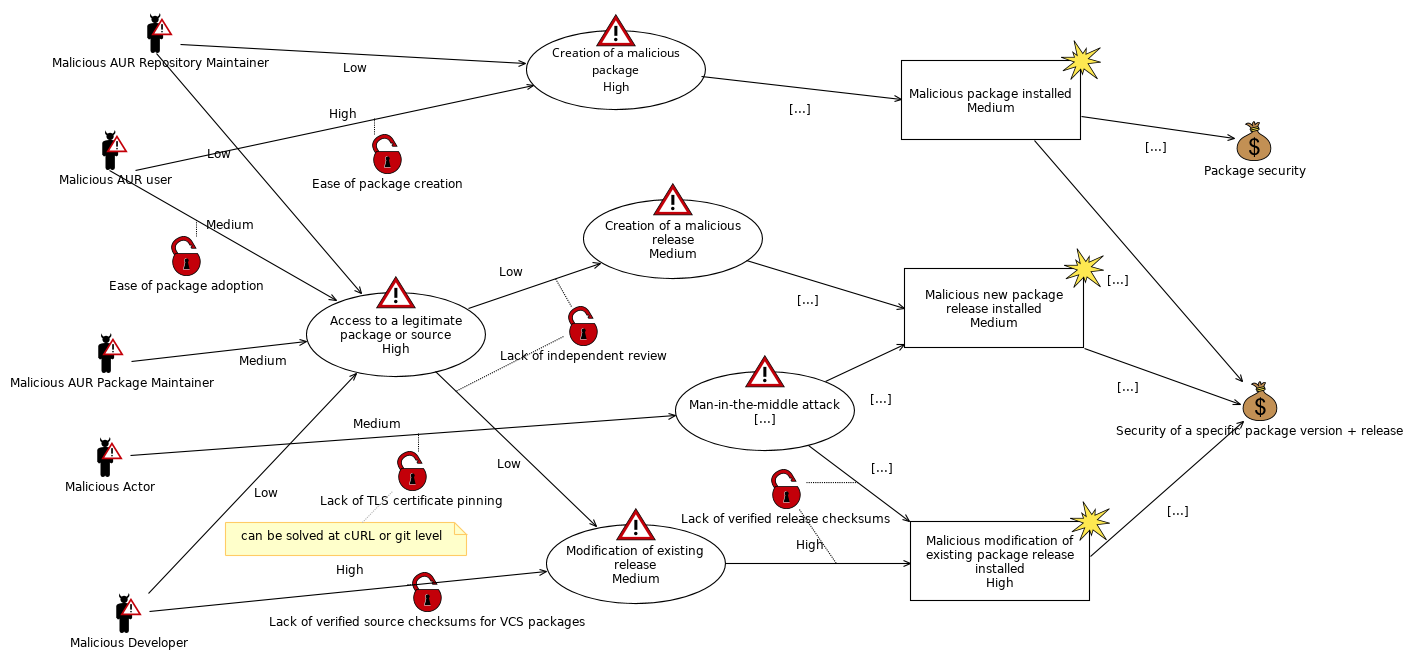
\includegraphics[width=\paperwidth]{img/threat.png}
	\caption[Threat Assessment]{Threat Assessment of the Arch User Repository}
	\label{fig:threat}
\end{figure}

\subsection*{Concrete Attack Scenarios}
We used the CORAS \cite{Dahl:2007} threat modeling language to arrange the security issues in such a way that concrete attack scenarios are intuitive to comprehend and retrace. The resulting threat diagram can be seen in Figure~\ref{fig:threat}.

Many of the AUR's security issues exist by design and are only included for completeness. However, several issues lead to the same situations; This means that security issues further along the right of the diagram tend to be more promising candidates in the search for solvable problems.

This knowledge leads to two concrete attack scenarios that could be preempted without redesigning the AUR, which are outlined below.

% Threats:
\subsection*{Tampered VCS Sources: Malicious Upstream}
In some cases, the user is not adequately protected against malicious (or compromised) upstreams:

The AUR supports so-called \emph{VCS packages} \cite{wiki:VCSPackages}, which download sources from a version control system, such as Git or Mercurial, instead of downloading a fixed archive. This relieves the maintainer from updating his \texttt{PKGBUILD} for every new commit.
\texttt{makepkg} will even automatically calculate the up-to-date version number using e.g. tags and commit numbers.

VCS packages were primarily designed to simplify the installation of up-to-date packages from source, and they do that very well; But they also introduce a big security issue:
Since the \texttt{PKGBUILD} must not be updated between versions, it cannot contain checksums for the new version, either.
This means that users don't have a way to verify the authenticity of the source that they are downloading, unless they can trust the upstream himself, meaning that no-one will notice if the upstream is compromised or makes malicious changes. There is no way to defend against this except to manually audit the upstream sources, which should primarily be the maintainers responsibility.

\subsection*{Tampered Packages: Malicious Maintainer}
Users are also not adequately protected against malicious maintainers:

Because it's so easy to gain access to a package, e.g. by adopting an orphan or simply by creating it, and nothing is verified or audited before publication, It's easy for a malicious agent to modify a package.
And because the \texttt{PKGBUILD} is not signed or hashed, users will not notice if the build instructions for a specific package version were modified. This allows targeted attacks:

If the time at which a target will update his machine is known and one has access to an AUR package which he is expected to update, malicious code can somehow be introduced into the corresponding \texttt{PKGBUILD} within that update window.
This could be as simple as changing the checksum if one also has access to the upstream source code (even a very careful user has no chance of noticing this attack), or executing innocuous code in the install file or \texttt{PKGBUILD} itself.

The malicious change could be reverted immediately afterwards. If the time frame is short, no other AUR user (and thus, \emph{no-one}) would ever notice.
One could only defend against this with a good local trust model, such as that possible with \texttt{bauerbill}, or manual cryptographic verification of the git commit to the AUR --- assuming that the maintainer signs his commits, which is only very rarely the case.

  % BENNETT
  \section{The Solution}
    \subsection{Core Solution}
    % extend Workflow2.jpeg  and integrate workflow.png int the discription ||| LUKAS
    % Mention that we appear to be the first to use a blockchain like this
    \subsection{Detailed Description}
    % aursec-init   ||| LUKAS
    % aursec systemd services  ||| BENNETT
    % aursec{,-hash,-verify-hashes}   ||| BENNETT
    % aursec-chain	||| LUKAS
    % TODO: what else
    \subsection{Terminal User Interface}
    % TUI  ||| LUKAS
    % TODO: what else?
    \subsection{Project Management}
    % Timeline  ||| LUKAS
    % TODO: What else?

  \section{Things we Learned}
  % Ethereum - Solidity
  % RPC API
  % Bash as a programming language
  % Python - Urwid
  % TODO: WHAT ELSE?

  \section{Evaluation}
  % We can probably already talk about our own experience? Our Data/ Data from outside ?

  %%% Content ends here
  \pagebreak
  % TODO: preferrably cite english pages
  \bibliographystyle{plain}
  \bibliography{Literature.bib}

\end{document}
